\documentclass[a4paper]{article}
\usepackage[margin=1in]{geometry} % 设置边距,符合Word设定
\usepackage{ctex}
\usepackage{graphicx} %插入图片的宏包
\usepackage{float} %设置图片浮动位置的宏包
\usepackage{subfigure} %插入多图时用子图显示的宏包
\usepackage{lipsum}
\usepackage{minted}% 语法高亮和代码样式设置方面更加强大和灵活
\usepackage{listings}% 引入listings包,用于在文档中插入代码,并可自定义代码样式
\usepackage{caption}



\title{奥运会项目评估模型:随机森林回归在体育决策中的应用}
\author{ 郭润恒 \ 杨子程 \ 邱信阳}
\date{\today}

\begin{document}
    \maketitle


\begin{abstract}
    % 随着奥运会项目的不断演变,国际奥林匹克委员会(IOC)面临着选择哪些运动项目(SDEs)加入2032年夏季奥运会的挑战。本研究旨在通过构建一个数学模型,根据IOC的标准评估SDEs,以提供有依据的推荐。该模型综合考虑了受欢迎度和可达性、性别平等、可持续性、包容性、相关性与创新以及安全与公平竞争等多个维度。通过对历史数据的分析和模型的构建,我们识别出可能在2032年布里斯班奥运会上新增或重新引入的SDEs,并对其优先级进行排序。本研究的结果将为IOC提供决策支持,确保奥运会项目的相关性和影响力。
    随着奥运会项目的不断演变,国际奥林匹克委员会(IOC)面临着选择哪些运动项目(SDEs)加入2032年夏季奥运会的挑战。
    \par 针对任务1,我们根据IOC标准,通过在网上查找多方面的资料并参考权威数据,对这些运动的受欢迎度和可达性、性别平等性、可持续性、包容性、相关性与创新性、安全与公平竞争性、新建更多项目的可能性共七个维度因素,在0-1之间进行了评分。
	\par 针对任务2,我们对1948-2020年项目数量的变化表格进行分析,在排除了一些受极端事件影响、较多年份数据残缺的项目后,选出33个项目的数据,利用Python语言进行了数据的可视化操作。然后,我们使用一次线性拟合,分析从1948到2020年的项目数变化的规律性特征。以七个维度作为自变量,线性拟合的斜率作为因变量,训练了一个随机森林回归模型。
    \par 针对任务4,我们利用训练好的随机森林回归模型,识别了三个可能在2032年布里斯班奥运会上新增或重新引入的 SDEs ,并确定其优先推荐的顺序。
\end{abstract}
\tableofcontents
\section{Introduction}
\subsection{Background}     
\subsection{Our Work}
\subsection{Data Pre-processing}


\section{Assumptions}
% 我们通过在网上查找多方面的资料并参考权威数据,最后对33个项目的七个维度进行了评分,结果如下:

展示表格

\section{Abbreviation and Definitions}
\section{The Evaluate Model}
\subsection{线性拟合模型}
We first excluded some items with poor data, such as 1, 2, and 3.Finally, we chose data from 33 items to train our model, 20\% of them are randomly decided as test dataset for model, and two of them are for manually test.
We then used one linear fit to the number of projects from 1948 to 2020 for each project:
\captionsetup[listing]{labelformat=empty}
\begin{figure}[H] %H为当前位置,!htb为忽略美学标准,htbp为浮动图形
    \centering %图片居中
    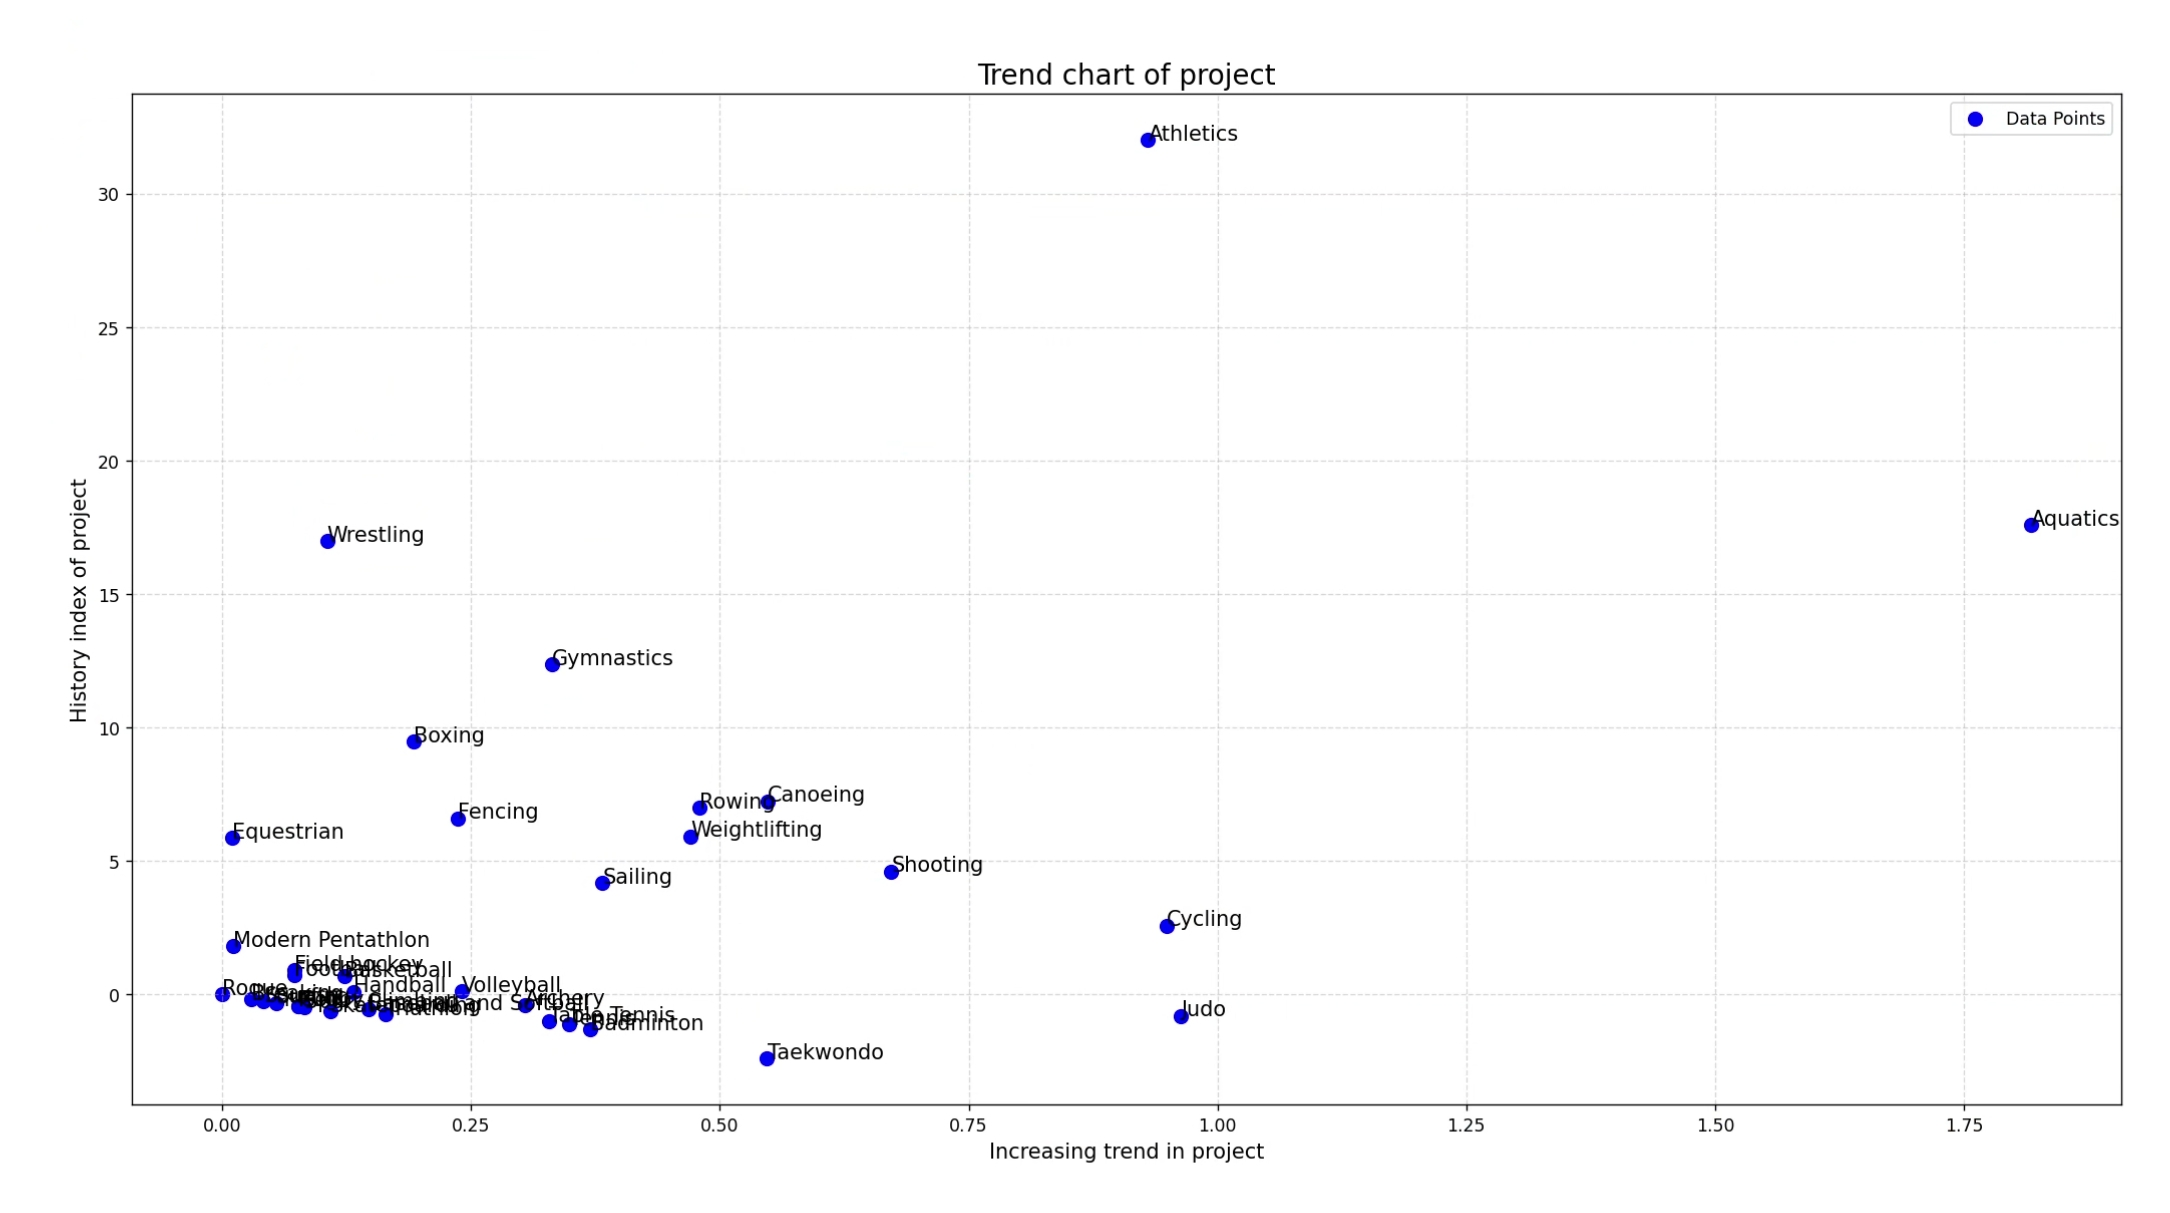
\includegraphics[width=0.7\textwidth]{TrendChartOfProject} %插入图片,[]中设置图片大小,{}中是图片文件名
    \caption{Main name 2} %最终文档中希望显示的图片标题
    \label{Fig.main2} %用于文内引用的标签
    \end{figure}

\subsection{随机森林回归}
\subsubsection{Introduction}
%TODO: 随机森林回归的定义

% 我们以七个维度和作为自变量,线性拟合的斜率作为因变量,训练了一个随机森林回归模型。

\subsubsection{Implementation}
We used the random forest fitting algorithm from the sklearn module of python.
% Code
\begin{listing}[htb]\caption{STH}\label{code:processdweet}
    \begin{minted}{python3}
        model = RandomForestRegressor(n_estimators=100, random_state=42)
        model.fit(X_train, y_train)
\end{minted} 
\end{listing}


\subsubsection{Result Analysis}
In the test set, our model achieved an R Square error of 0.6 and a mean square error of 0.12, making the regression training basically successful.

We used this model to predict data outside of the training and test sets

\begin{table}[]
    \begin{tabular}{lllllllll}
    Name      & Popularity and Accessibility & Gender Equity & Sustainability & Inclusivity & Relevance and Innovation & Safety and Fair Play & Basis & Rank        \\
    Wrestling & 0.7                          & 0.6           & 0.8            & 0.8         & 0.5                      & 0.8                  & 0     & 0.105263158 \\
              &                              &               &                &             &                          &                      &       &             \\
              &                              &               &                &             &                          &                      &       &            
    \end{tabular}
    \end{table}

结果表明,我们的模型在预测项目数量的增长上取得了成功。



\section{对SDE项目的预测}
我们对某个SDE项目进行了评分,输入我们的模型,得到了如下结果

我们认为 它的增长是xxx
\subsubsection{Background of This Problem}
\subsection{Efficiency and Robustness}
\section{Sensitivity Analysis}
\section{Strengths and Weaknesses}
\subsection{Strengths}
\subsection{Weaknesses}
\section{Conclusion}
Hello world!test123
\end{document}  